% !TEX TS-program = LuaLaTeX
\documentclass[10pt, oneside, a4paper]{article}

\usepackage[T1]{fontenc}
\usepackage{lmodern}
\usepackage{xcolor}
    \definecolor{gray} {HTML}{363636}
    \definecolor{red}  {HTML}{950009}
    \definecolor{green}{HTML}{0E610A}
    \definecolor{blue} {HTML}{020069}
\usepackage{fontspec}
    \setsansfont{Arial}
\usepackage{amsmath}
\usepackage{titlesec}
    \titleformat*{\section}      {\color{gray}\large\bfseries\sffamily}
    \titleformat*{\subsection}   {\color{gray}\large\bfseries\sffamily}
    \titleformat*{\subsubsection}{\color{gray}\large\bfseries\sffamily}
\usepackage{geometry}
    \geometry{scale={0.75,0.85}}
\usepackage{siunitx}
    \sisetup{locale=FR}
    \sisetup{math-micro=\text{µ},text-micro=µ} % fix
\usepackage{graphicx}
\usepackage{caption}
    \captionsetup{labelfont={bf,sf,color=gray}}
\usepackage{pdfpages}
\usepackage{caption}

\usepackage{mwe} % For dummy images
\usepackage{subcaption}

\usepackage{fancyhdr}
\pagestyle{fancy}
\fancyhead[R]{}
\fancyfoot[L]{Thomas Anizet}
\fancyfoot[C]{}
\fancyfoot[R]{\thepage}


% Keep lasts
\usepackage[french]{babel}
    \frenchsetup{SmallCapsFigTabCaptions=false}
\usepackage[expansion]{microtype}
\usepackage[luatex, backref]{hyperref}
    \hypersetup{unicode, colorlinks, breaklinks, urlcolor=red,
                bookmarksopen, bookmarksnumbered}

\renewcommand{\UrlFont}{\small}
\renewcommand{\arraystretch}{1.1}
\setlength{\parskip}{2mm}

\begin{document}


%%%%%%%%%%%%%%%%%%%%%%%% Table des matières
\tableofcontents
\newpage

%%%%%%%%%%%%%%%%%%%%%%%% Introduction

\phantomsection
\section*{Introduction}
\addcontentsline{toc}{section}{Introduction}

Candidat "Officier de carrière" à l’\textbf{\textit{École Royale Militaire}} (ERM), je suis actuellement ma formation académique à l’\textbf{\textit{École Centrale des Arts et Métiers}} (ECAM) en option électronique. \\ \\
Durant notre 2ème année de Master, les étudiants doivent réaliser un stage d’immersion en entreprise d’une durée de 6 semaines. Ce stage consiste, entre autres, à s’insérer dans une entreprise afin d’y découvrir différents aspects tels que l’organisation générale d’une entreprise, son management, son contexte social, son insertion économique, ses aspects techniques et ses produits. Il a également pour but de se familiariser au travail quotidien de l’ingénieur en participant à diverses activités. \\ \\
Ayant réalisé mon stage de 3ème Bachelier chez \textbf{\textit{AIRBUS DS SLC}} sur le site de Diegem et de Elancourt, il était important pour moi de saisir la chance et l’opportunité de découvrir une nouvelle entreprise renommée à travers le monde. C'est ainsi que je décidai de réaliser mon stage chez \textit{\textbf{THALES} Telecommunications Belgium} sur le site de Tubize. 

\newpage

%%%%%%%%%%%%%%%%%%%%%%%% Partie 1 - Environnement de stage %%%%%%%%%%
\section{Environnement de stage}
Cette section a pour objectif de décrire l'entreprise à différents points de vue. Tout d'abord, une description de la structure de l'entreprise (dont l'équipe dans laquelle se trouve le stagiaire) et de ses objectifs est reprise. Ensuite, sont détaillées succontement la gestion de production mais aussi la gestion marketing, la gestion financière et la gestion des ressources humaines. Enfin, un descriptif de la cellule qualité clôturera ce premier point.

\subsection{Structure de l'entreprise}
C'est donc chez \textbf{\textit{Thales}} \textit{Telecommunication Belgium} que je me suis rendu pour réaliser mon stage d'immersion en entreprise. 

\subsection{Objectifs de l'entreprise}


\subsection{Equipe du stagiaire}


\subsection{Gestion de production}


\subsection{Gestion marketing}


\subsection{Gestion financière}


\subsection{Gestion des ressources humaines}


\subsection{Politique QHSE}


\newpage
%%%%%%%%%%%%%%%%%%%%%%%% Partie 2 - Objectifs du stage %%%%%%%%%%%%%
\section{Objectifs du stage}
\label{sec:objectifs}

L'objectif de ce stage était d'introduire l'ensemble des notions élémentaires, nécessaires pour la réalisation du \textit{Travail de Fin d'Étude} (TFE). Ce travail de fin d'étude qui allait se poursuivre durant 6 mois à compter du mois de Novembre 2018. Dans un premier temps, une définition des notions théoriques est abordée. Ensuite, un exemple ou une simulation est mise en oeuvre afin d'appuyer le concept théorique.\\ \\
La liste ci-dessous reprend l'ensemble des objectifs fixés et réalisés durant les 6 semaines de stage : 
\begin{description}
\item[1. Chiffrement] 
\item[2. L'algorithme AES (\textit{Advanced Encryption Standard})]
\item[3. \textit{Side-Channel Attacks} (attaques par canal auxiliaire)]
\item[4. Simulation d'un tracé et d'une attaque par canal auxiliaire sur MATLAB] 
\item[5. Statistiques et t-test] 
\item[6. Simulation d'un t-test sur MATLAB] 
\end{description}
Ces différents objectifs sont décrits dans la section \ref{sec:Projet} \textit{"Projet du stage"}.

%%%%%%%%%%%%%%%%%%%%%%%% Partie 3 - Projet du stage %%%%%%%%%%%%%
\section{Projet du stage}
\label{sec:Projet}

Cette section décrit l'ensemble des objectifs, cités à la section \ref{sec:objectifs}, fixés pour le stage. 

%%%% PARTIE 3.1
\subsection{Notions  de chiffrement}

Les systèmes de sécurité modernes utilisent des algorithmes de chiffrement pour assurer la disponibilité, la confidentialité et l'intégrité de données. Ces algorithmes de chiffrement sont en réalité des fonctions mathématiques qui prennent typiquement : 
\begin{itemize}
\item  2 paramètres en entrée : un \textbf{\textit{message clair}} (nommé \textit{plaintext} en anglais) et une \textbf{\textit{clé de chiffrement}} (nommée \textit{key} en anglais).
\item 1 paramètre en sortie : le \textbf{\textit{message chiffré}} (nommé \textit{ciphertext} en anglais). \\
\end{itemize}
Le procédé transformant les données claires en entrée en données chiffrées en sortie est appelé le \textbf{\textit{chiffrement}}.
Ce procédé est réalisé grâce à un \textbf{\textit{algorithme de chiffrement}} utilisant une clé de chiffrement et diverses opérations mathématiques. Il est important de préciser que tous les détails décrivant le fonctionnement d'un algorithme sont disponibles publiquement, seule la clé de chiffrement doit rester secrète. En effet, la sécurité offerte par un algorithme de chiffrement ne doit pas dépendre du secret de son implémentation. Un bon algorithme est un algorithme dont on ne parviendra pas à déchiffrer les données chiffrées. Lorsque la clé d'un algorithme est trouvée, le déchiffrement des données confidentielles peut être réalisé. On dit que l'algorithme de chiffrement est \textbf{\textit{cassé}}.

La figure \ref{fig:chiffrement} ci-dessous présente le principe de fonctionnement d'un algorithme de chiffrement.

\begin{figure}[htbp]
    \centering
    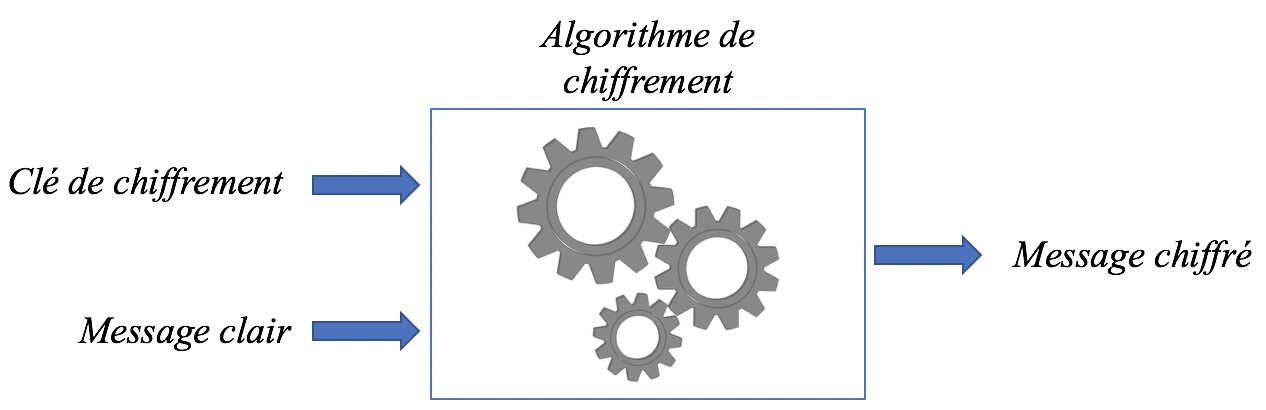
\includegraphics[width=0.7\textwidth]{image/chiffrement}
    \caption{L'algorithme de chiffrement, caractérisé par diverses opérations mathématiques, utilise une clé de chiffrement en entrée pour chiffrer un message clair. Cela produit un message chiffré, non compréhensible pour une personne ne connaissant pas la clé de chiffrement.}
    \label{fig:chiffrement}
\end{figure}

\newpage

Nous distinguons 2 types d'algorithmes de chiffrements : 
\begin{itemize}
\item \textbf{\textit{Chiffrement symétrique}} : Le chiffrement est dit symétrique lorsque le procédé de chiffrement (algorithme) utilise une seule clé, appelée \textit{clé secrète}. Par convention, ce type de chiffrement permet à la fois de chiffrer et de déchiffrer des messages à partir d'une seule et unique clé. Le désavantage de ce typer de chiffrement est que si une personne parvient à subtiliser la clé publique, elle sera en mesure de déchiffrer tout message qu'elle intercepte.  \\
\textit{Exemple} : L'algorithme AES. Une explication plus détaillée de cet algorithme est reprise à la section \ref{sec:AES}
\item \textbf{\textit{Chiffrement asymétrique}} : Le chiffrement est dit asymétrique lorsque le procédé de chiffrement (algorithme) utilise 2 clés : une \textit{clé publique} et une \textit{clé privée}. Par convention, la clé publique est la clé de chiffrement du message clair, elle peut être communiquée sans aucune restriction tandis que la clé privée est la clé de déchiffrement du message chiffré, elle ne doit être communiquée sous aucun prétexte. Le fonctionnement est le suivant : Avec une clé publique, l'expéditeur code, dans un algorithme de chiffrement donné, un message. Ce message, une fois transmis, ne pourra être déchiffré que par le destinataire, détenteur de la clé privée. \\
\textit{Exemple} : L'algorithme RSA. \\
\end{itemize}

Les figures \ref{fig:symétrique} et \ref{fig:asymétrique} ci-dessous présentent les principes de fonctionnement des chiffrements symétriques et asymétriques respectivement.

\begin{figure}[htbp]
    \centering
    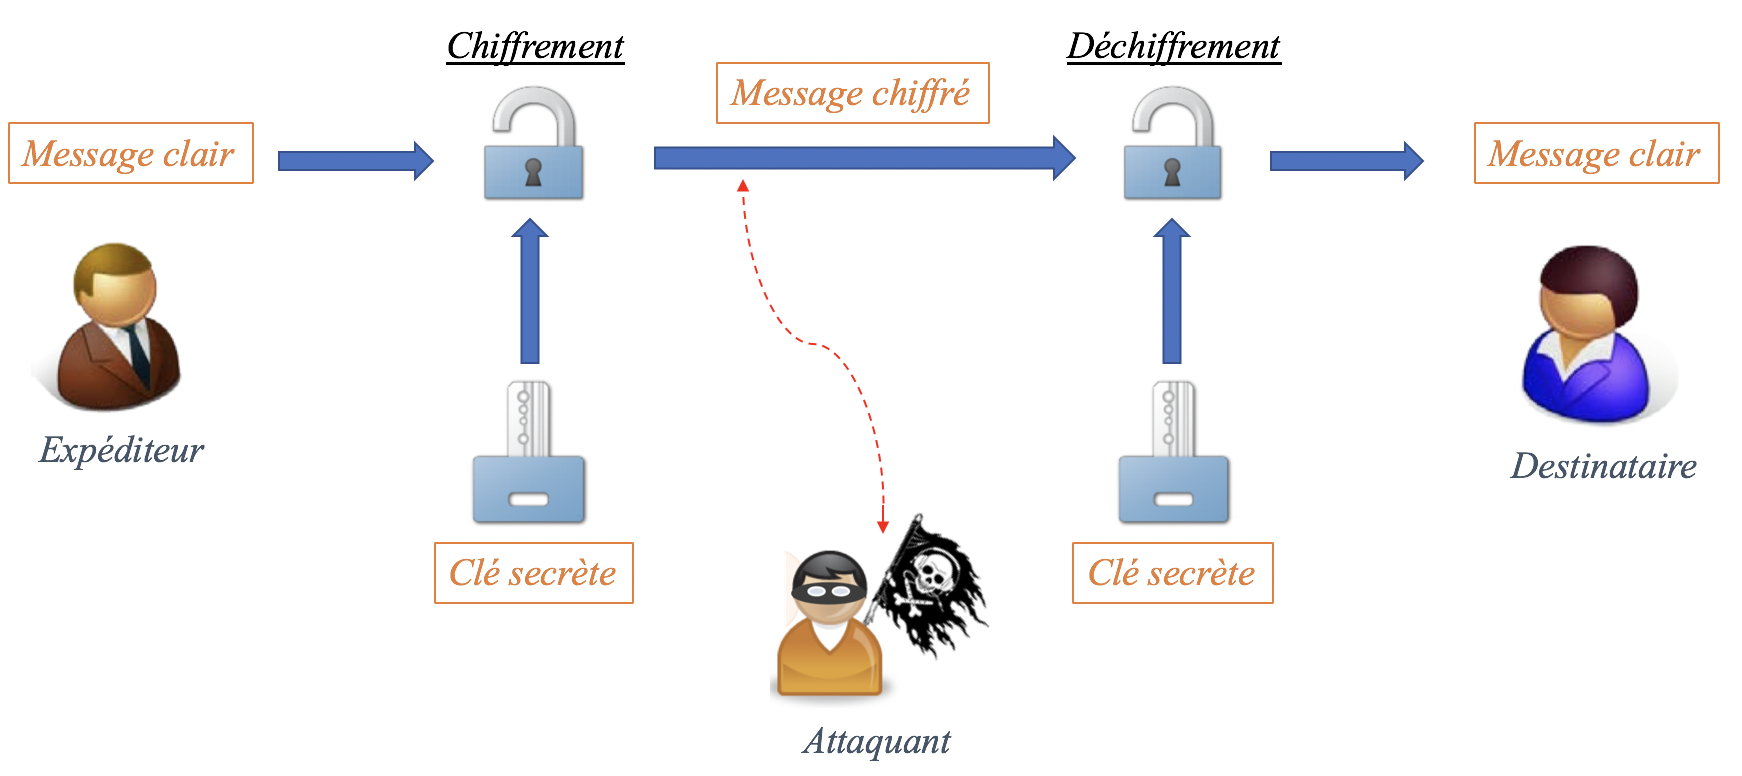
\includegraphics[width=0.65\textwidth]{image/symetrique}
    \caption{Chiffrement symétrique : Une seule clé est utilisée pour chiffrer et déchiffrer les messages.}
    \label{fig:symétrique}
\end{figure}

\begin{figure}[htbp]
    \centering
    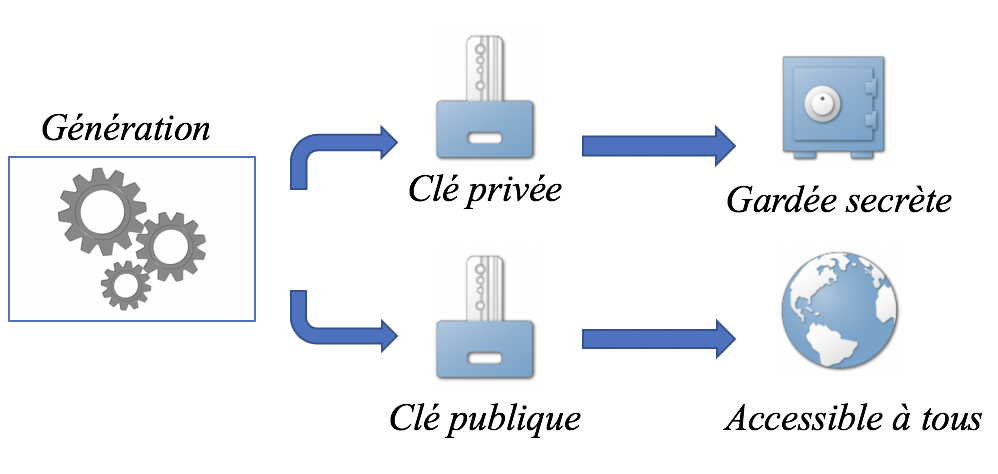
\includegraphics[width=0.38\textwidth]{image/cle_asymetrique}
    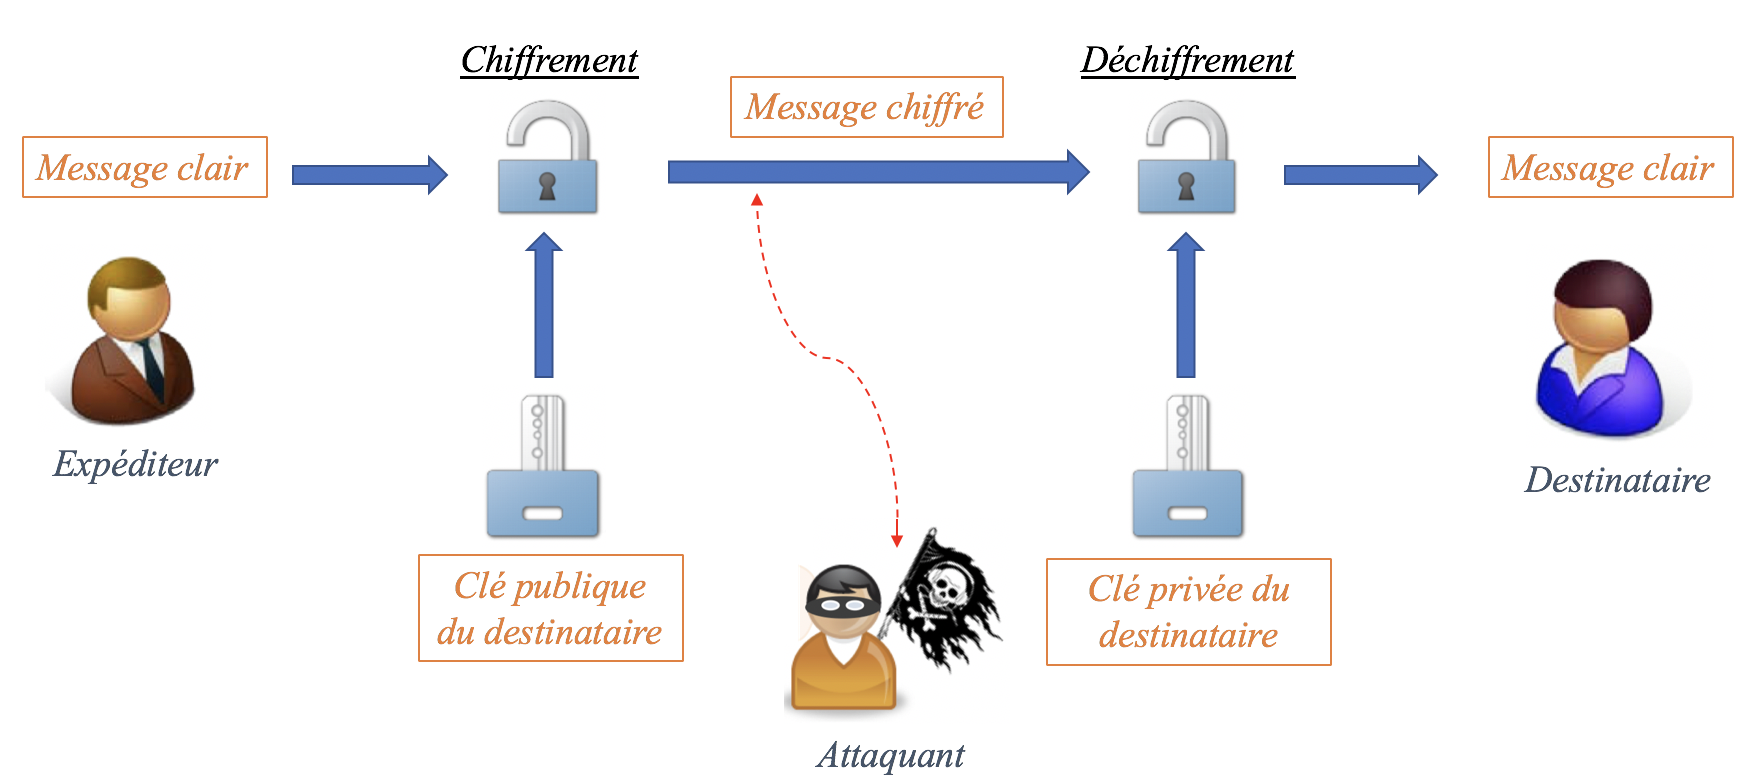
\includegraphics[width=0.7\textwidth]{image/asymetrique}
    \caption{Chiffrement asymétrique : Un clé publique est utilisée pour chiffrer le message et une clé privée est utilisée pour le déchiffrer.}
    \label{fig:asymétrique}
\end{figure}


Que ce soit pour un algorithme de chiffrement symétrique ou asymétrique, la clé de chiffrement doit être stockée sur un support physique. Ce support, appelé \textit{device cryptographique}, doit être suffisamment sécurisé que pour contenir de manière protégée la clé. Ainsi, un \textbf{\textit{device cryptographique}} est un device qui implémente des algorithmes de chiffrement et qui stocke des clés de chiffrement.

\subsection{Algorithme \textit{AES} (\textit{Advanced Encryption Standard})}
\label{sec:AES}

En 1997, le NIST (\textit{National Institute of Standards and Technology}) décida qu'il était temps de développer un nouveau standard d'algorithme de chiffrement. Ce nouveau standard, nommé \textbf{AES} (pour \textit{Advanced Encryption Standard}), était appelé à remplacer l'ancien standard de chiffrement, l'algorithme DES (pour \textit{Data Encryption Standard}). Pour ce faire, le NIST organisa un concours cryptographique, les chercheurs du monde entier furent invités à soumettre leurs propositions. En Octobre 2000, Le NIST annonça le vainqueur du concours : l'algorithme de Rijndael, du nom de ses concepteurs Joan Daemen et Vincent Rijmen, tous deux de nationalité belge.

L'algorithme de Rijndael, désormais plus connu sous le nom d'algorithme AES, est un algorithme de chiffrement symétrique par blocs. C'est-à-dire que les données sont traitées par blocs de 128 bits. La clé secrète peut posséder différentes longueurs : 128 bits (AES-128), 192 bits (AES-192) ou encore 256 bits (AES-256). À noter qu'en théorie, plus la taille de la clé est élevée, moins il y a de chance de casser l'algorithme cependant avec les side-channel attacks, le problème peut vite être contourné. \\ La description qui suit est basée sur l'algorithme AES-128 bits, c'est-à-dire que la clé de chiffrement a une taille de 128 bits.

L'AES-128 a donc pour rôle de chiffrer des blocs de données de 128 bits avec une clé de 128 bits. Les données et la clé sont représentés par une matrice où chaque élément de la matrice correspond à un byte (un octet soit 8 bits). Étant donné que 128 bits correspond à 16 bytes, la matrice de données, au même titre que la matrice de clé, correspond à une matrice de 4 lignes et 4 colonnes (formant ainsi les 4x4 soit 16 bytes). Une matrice particulière (de taille 4x4) appelé STATE contient l'ensemble des résultats intermédiaires résultant des diverses opérations que subissent les données (depuis leur état initial). 

La figure \ref{fig:matrix} présente 3 matrices : la matrice de donnée (message clair initial de 128 bits), la matrice STATE (qui va contenir les résultats intermédiaires des données suite aux différentes opérations) et la matrice clé (clé de 128 bits).
\begin{figure}[htbp]
    \centering
    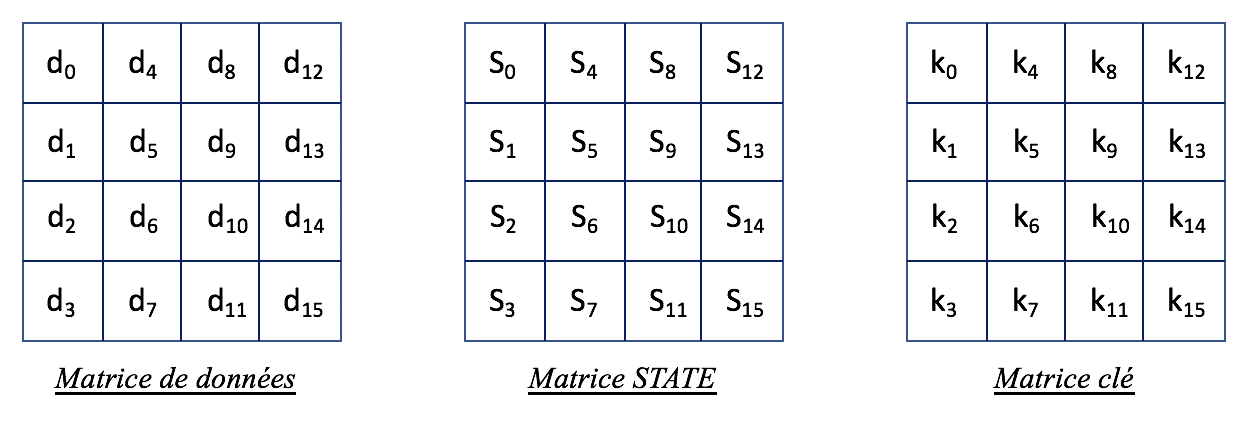
\includegraphics[scale=0.75]{image/matrix}
    \caption{Les 3 matrices utilisées par l'algorithme AES.}
    \label{fig:matrix}
\end{figure}

\textit{Remarque} : En réalité, la matrice de données est directement confondue avec la matrice STATE. Autrement dit, les premiers éléments à être placés dans la matrice STATE représentent les bytes de données. En résumé, on n'utilise que deux matrices durant le fonctionnement de l'algorithme AES : la matrice STATE et la matrice clé.

Par ailleurs, l'algorithme AES est caractérisé par une série de tours (\textit{rounds} en anglais) dépendant de la taille de la clé. Pour une clé dont la taille est 128 bits, on dénombre 10 tours (12 tours pour une clé de 192 bits et 14 tours pour une clé de 256 bits). Un tour est définit par 4 opérations appliquées succinctement sur la matrice STATE. Ces 4 opérations sont : \textit{AddRoundKey}, \textit{SubBytes}, \textit{ShiftRows}, \textit{MixColumns}. Elles sont appliquées à divers instants dans l'exécution de l'algorithme AES. La figure \ref{fig:AES} (page suivante) permet de visualiser l'ordre d'exécution chronologique de ces 4 opérations. 

\newpage

La figure \ref{fig:AES} ci-dessous présente le principe de fonctionnement général de l'algorithme AES-128.
\begin{figure}[htbp]
    \centering
    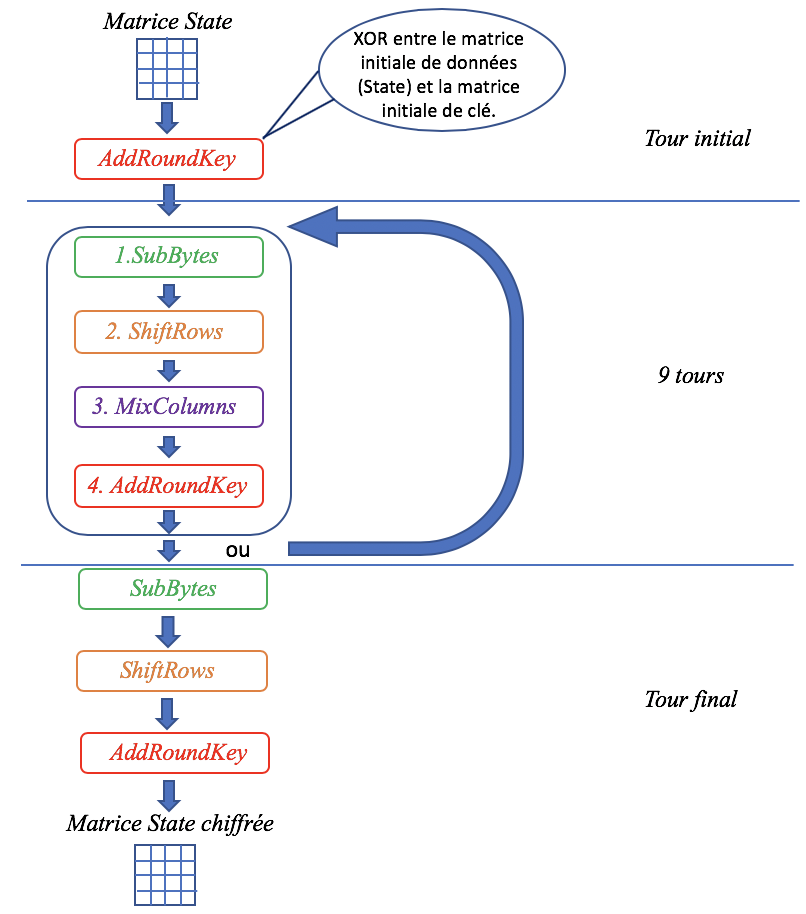
\includegraphics[scale=0.75]{image/AES}
    \caption{Principe de fonctionnement de l'algorithme AES-128.} 
    \label{fig:AES}
\end{figure}



\underline{\textbf{Fonctionnement :}} 

Initialement, 2 matrices vont être utilisées : la matrice STATE, contenant les données claires, et la matrice clé, contenant la clé secrète initiale. En effet, une première opération (\textit{AddRoundKey}) est appliquée sur ces deux matrices. Plus précisément, cette opération réalise un XOR (symbole \oplus) entre chaque élément de la matrice STATE et chaque élément de la matrice clé. Le résultat est ré-écrit dans la matrice STATE. La figure \ref{fig:XOR} ci-dessous présente le principe de fonctionnement de cette première opération :
\begin{figure}[htbp]
    \centering
    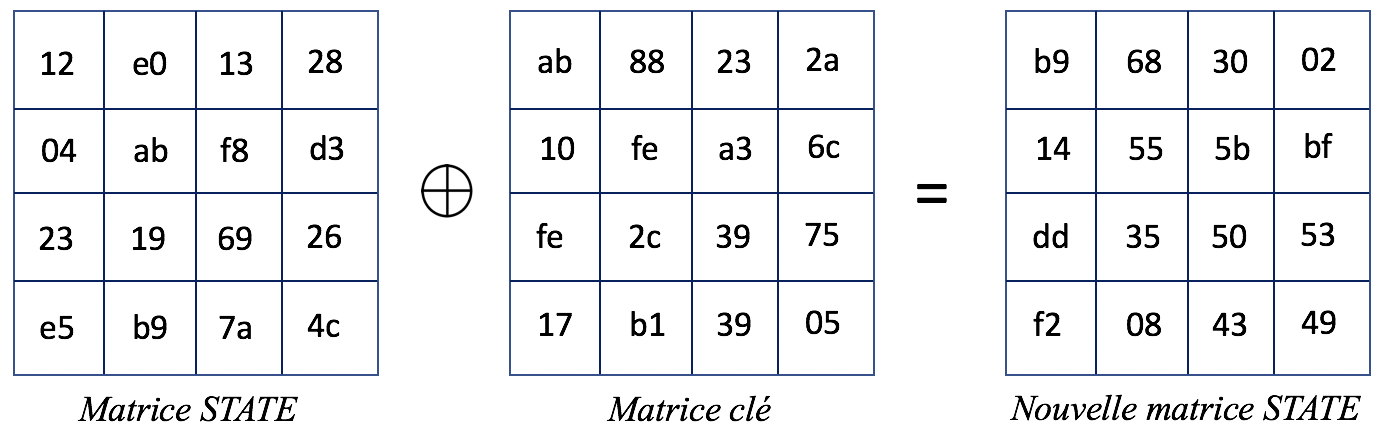
\includegraphics[scale=0.65]{image/XOR}
    \caption{Opération XOR entre la matrice STATE et la matrice clé.}
    \label{fig:XOR}
\end{figure}

\vspace{-0.5 cm}\hspace{-0.5 cm}Ensuite, une série de 4 opérations se répétant 9 fois (9 tours cycliques) est exécutée. Ces 4 opérations sont appliquées dans l'ordre suivant : \textit{SubBytes}, \textit{ShiftRows}, \textit{MixColumns}, \textit{AddRoundKey}. \\
Enfin, une fois les 9 tours exécutés, le dernier \textit{round} se lance exécutant 3 opérations : \textit{SubBytes}, \textit{ShiftRows} et \textit{AddRoundKey}. À la fin de ces 3 dernières opérations, une matrice de taille 4x4 présente le message chiffré de 128 bits.


\underline{\textbf{Description des 4 opérations :}} \\
\begin{description}
\item[1. SubBytes] : 
La figure \ref{fig:subByte} ci-dessous présente le principe de fonctionnement de l'opération \textit{SubBytes} :
\begin{figure}[htbp]
    \centering
    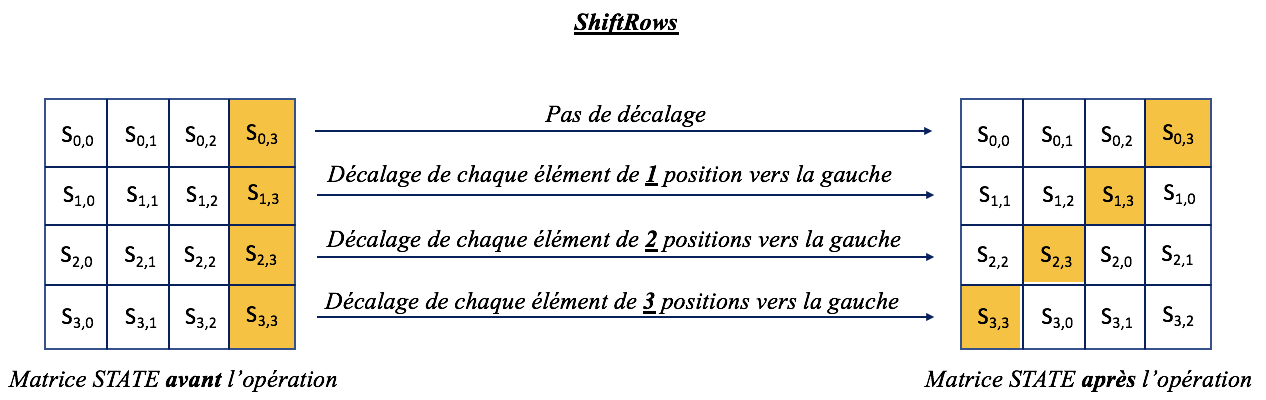
\includegraphics[width=1.05\textwidth]{image/ligne}
    \caption{Opération \textit{subBytes} exécutée sur la matrice STATE.}
    \label{fig:subByte}
\end{figure}

\item[2. ShiftRows] : Comme son nom l'indique, cette opération concerne les lignes de la matrice STATE. Cette opération réalise une permutation cyclique des octets sur les lignes de la matrice STATE. Plus précisément, \textbf{pour la \textit{i-ième} ligne, on décalera chaque élément de la matrice STATE de \textit{i} positions vers la gauche}, en considérant que la première a pour indice 0.
La figure \ref{fig:ligne} ci-dessous présente le principe de fonctionnement de l'opération \textit{ShiftRows} :
\begin{figure}[htbp]
    \centering
    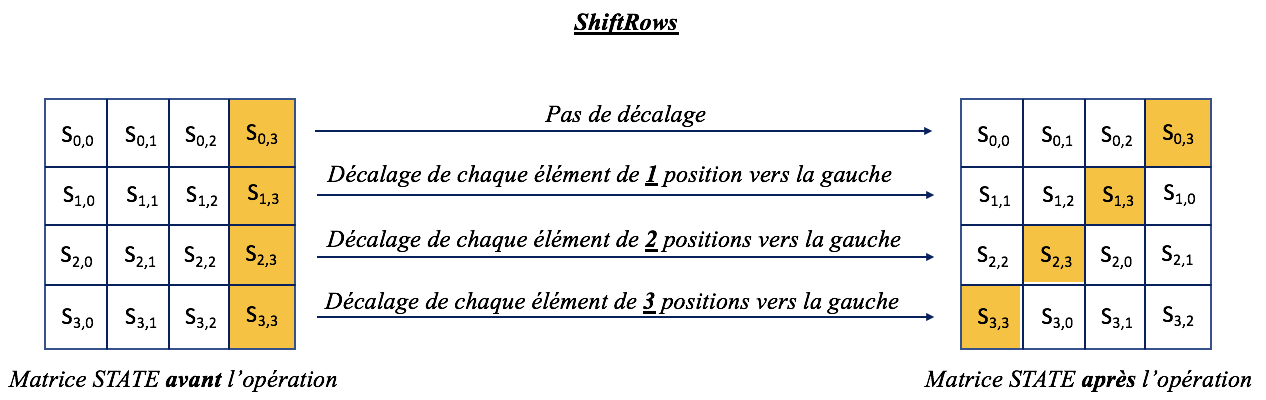
\includegraphics[width=1.05\textwidth]{image/ligne}
    \caption{Opération \textit{ShiftRows} exécutée sur la matrice STATE.}
    \label{fig:ligne}
\end{figure}

\item[3. MixColumns] : Comme son nom nom l'indique, cette opération concerne les colonnes de la matrice STATE. \textbf{Cette opération réalise un produit matriciel entre une matrice fixée (taille 4x4) définie ci-dessous (figure \ref{fig:colonne}) et un vecteur colonne (taille 4x1) de la matrice STATE}. Cela produit un nouveau vecteur colonne (taille 4x1) permettant de définir la nouvelle matrice STATE.
La figure \ref{fig:colonne} ci-dessous présente le principe de fonctionnement de l'opération \textit{MixColumns} :
\begin{figure}[htbp]
    \centering
    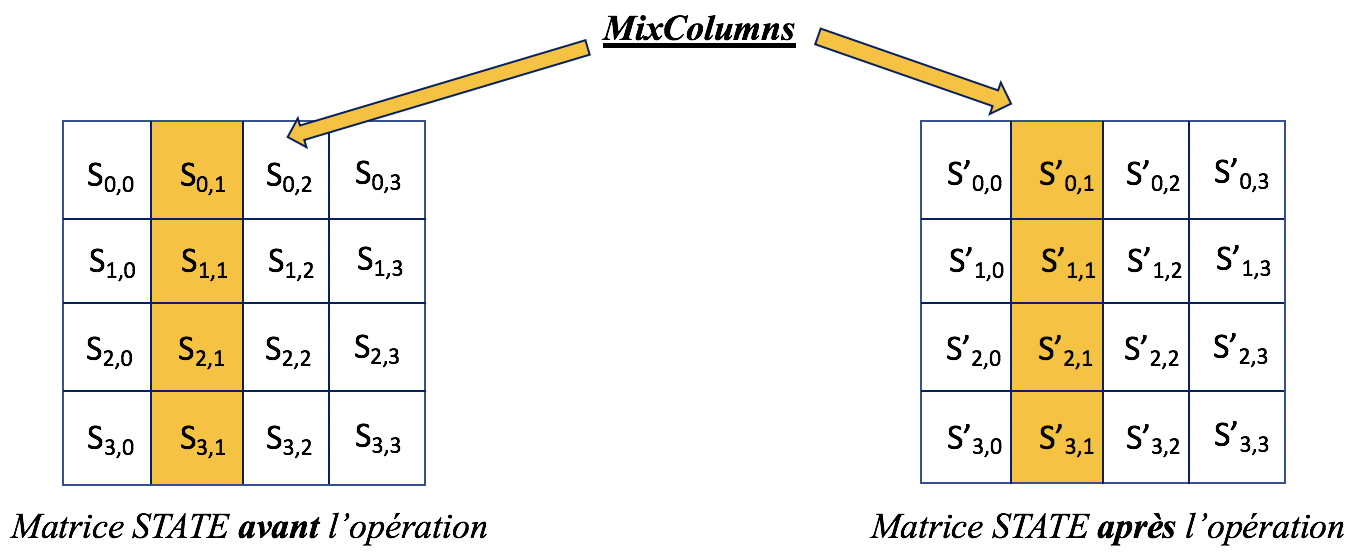
\includegraphics[scale=0.45]{image/colonne}
    \caption{Opération \textit{MixColumns} exécutée sur la matrice STATE.}
    \label{fig:colonne}
\end{figure}
\begin{figure}[htbp]
    \centering
    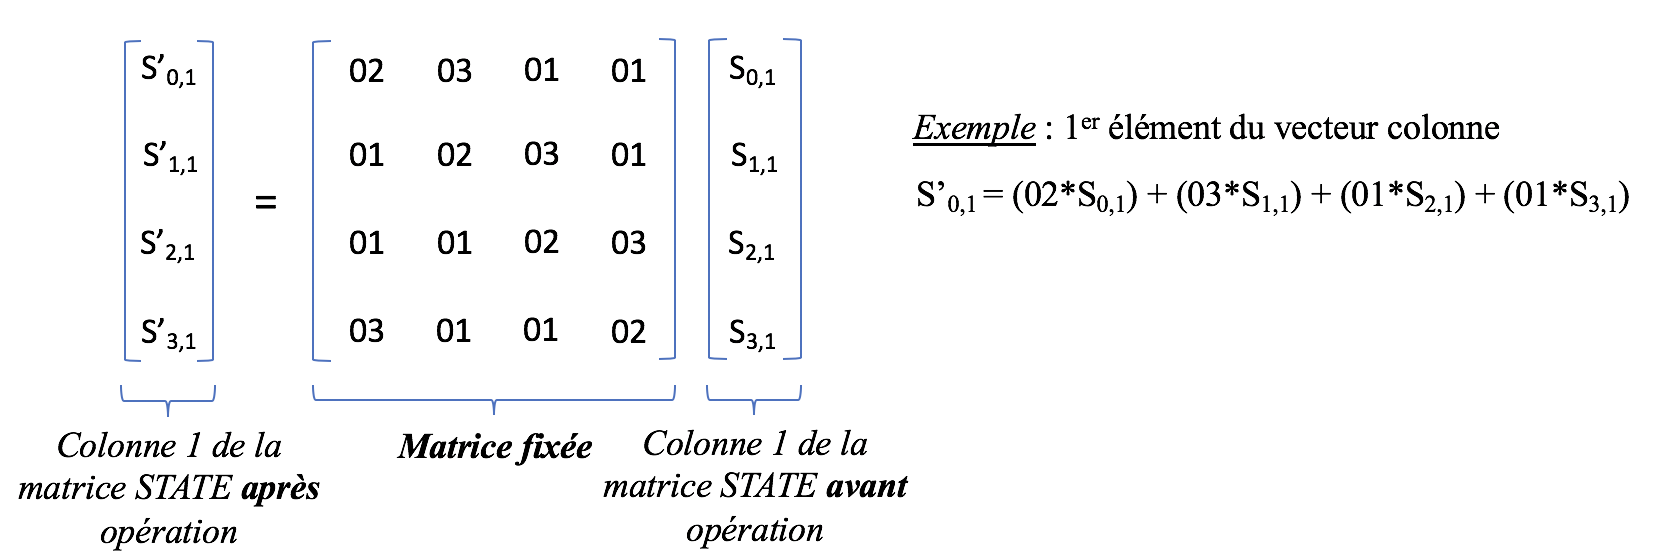
\includegraphics[width=1\textwidth]{image/colonnebis}
    \caption{Exemple de l'opération \textit{MixColumns} exécutée sur la deuxième colonne de la matrice STATE.}
    \label{fig:colonnebis}
\end{figure}

\item[4. AddRoundKey] :  La gestion des clés se fait au travers des fonctions addRoundKey et keyExpansion. AddRounkey réalise un XOR entre STATE et la clé courante (roundkey 8). Le résultat de ce XOR est placé dans STATE. Cette roundkey est dérivée de la clé secrète. On change de clé courante à chaque tour pour éviter d’utiliser toujours la même valeur ; cela rend la tâche d’attaquants plus difficile. KeyExpansion est là pour étendre la clé afin, comme nous l’avons dit plus haut, de ne pas utiliser la même clé à chaque tour. La taille de la clé, après avoir été étendue, est égale à la longueur d’un bloc multipliée par le nombre de tours plus un. En effet, il nous faut une clé différente par tour ; de plus, au début de l’algorithme, on exécute un addRounKey initial avant le premier tour. Pour AES-128 (10 tours et clé de 16 octets), la clé, après avoir été étendue, aura 176 octets. 16(10+1) = 176 octets. Le fonctionnement de KeyExpansion étant le même pour la construction de chaque sous-clé, nous allons voir comment on crée la première sous-clé à partir de la clé de départ ; ceci pourra se généraliser pour les autres clés en remplaçant « première sous-clé » par « i-ième sous-clé » et « clé de départ » par « sous-clé précédente ».
\end{description}


\newpage

\subsection{Notions de \textit{Side-Channel Attacks}}

A la fin des années 1990, une nouvelle contrainte pour la conception de système informatique a vu le jour : la sécurité matérielle. Bien souvent, la sécurité d'un système informatique s'appuie plus sur les concepts software que hardware. Cependant, un nouveau mode d'attaque s'est développé. Il s'agit d'attaques physiques, c'est-à-dire d'attaques réalisées sur le circuit électronique lui-même. Deux grandes familles d'attaques sont recensées : 
\begin{itemize}
\item \textbf{\textit{Attaques actives}} : Une attaque est dite active lorsque les entrées et/ou l'environnement du device cryptographique sont manipulés par l'attaquant en vue de produire un comportement anormal du device. La clé secrète est révélée en exploitant les données issues de ce comportement anormal. Cela peut être une variation de la tension du device, une injection de glitch d'horloge, etc. On distingue deux types d'attaques actives : 
\begin{itemize}
\item Les attaques actives \textbf{\textit{irréversibles}} qui conduisent à la destruction du device cryptographique. Ce type d'attaque est souvent réalisé pour connaître la conception physique d'un device. \textit{Exemple} : Découpage laser d’un circuit intégré.
\item Les attaques actives \textbf{\textit{pseudo-réversibles}} qui n’entrainent pas forcément la destruction du device cryptographique, mais qui sont souvent tout de même invasives puisqu’elles nécessitent la préparation du circuit (découpe partielle du boitier du circuit intégré par exemple). Un exemple typique de ce type d'attaque est ce qu'on appelle les attaques en fautes. Le principe est d'introduire volontairement des fautes dans le circuit (exemple : Injection de rayon laser, injection de glitch d’horloge, etc.). Les fautes ainsi créées peuvent entrainer le circuit dans des modes de fonctionnement conduisant à des erreurs. Ces erreurs peuvent ensuite être exploitées pour déterminer la clé.
\end{itemize}
\item \textbf{\textit{Attaques passives}} : Une attaque est dite passive lorsque l'attaquant exploite l'analyse, en fonctionnement normal, d'informations s'échappant d'un device cryptographique. Cela peut être l'analyse de la consommation de puissance, l'analyse temporelle, l'analyse par rayonnement électromagnétique, etc. C'est ce type d'attaque qui sera détaillé tout au long de ce stage et durant la réalisation de TFE. \\
\end{itemize}

La figure \ref{fig:attaques} ci-dessous résume les différents types d'attaques physiques possibles.
\begin{figure}[htbp]
    \centering
    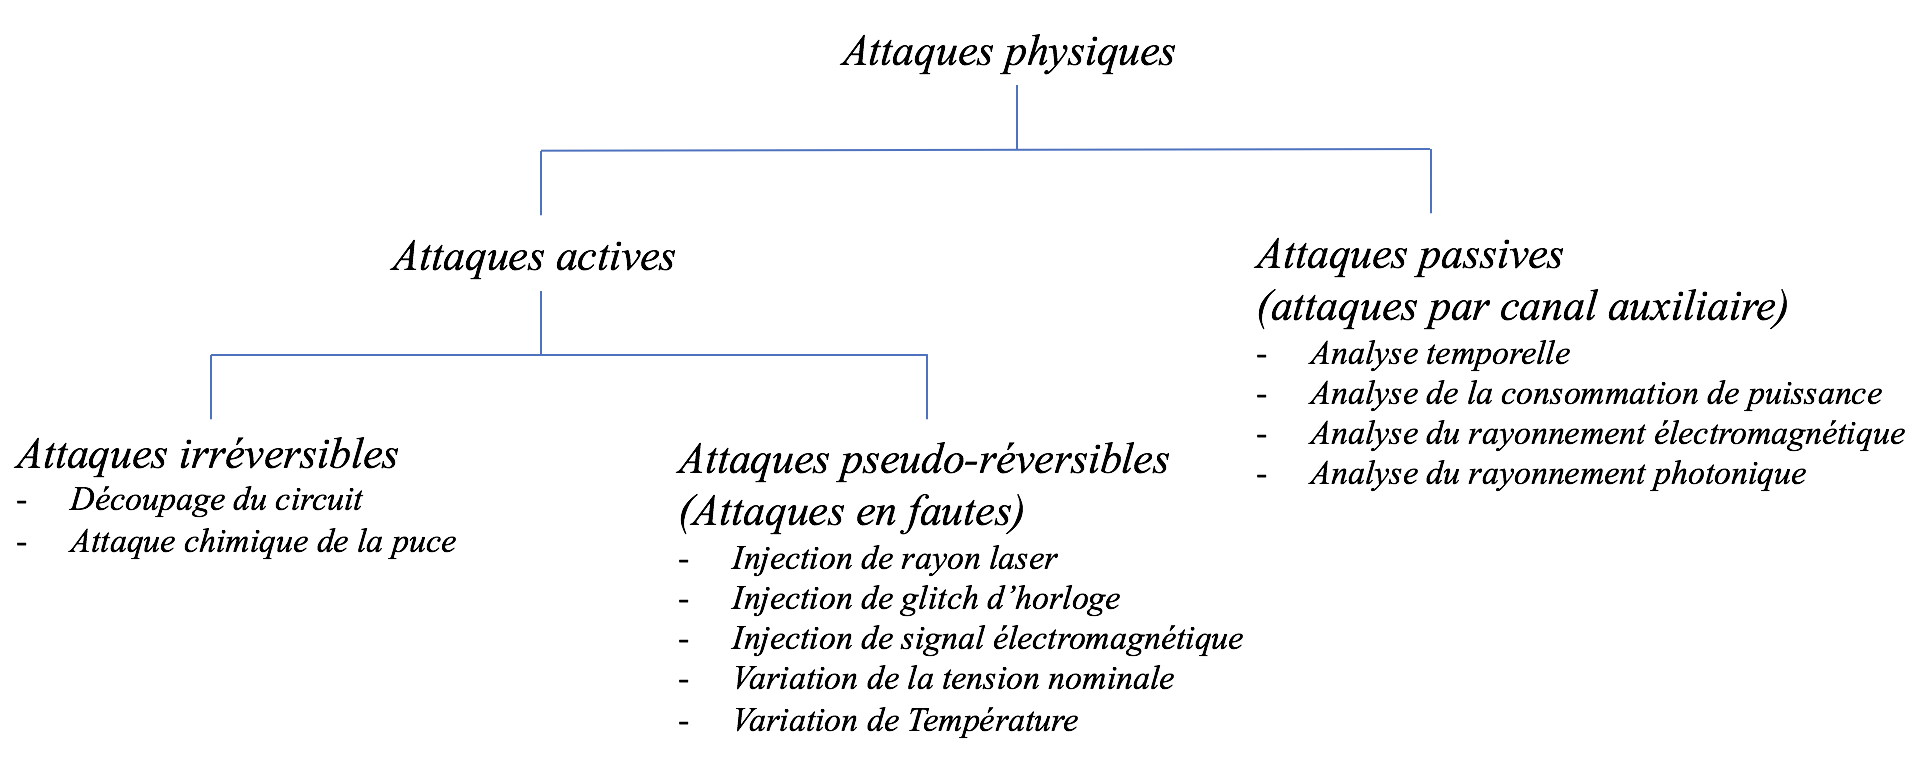
\includegraphics[width=0.9\textwidth]{image/attaques}
    \caption{Les 2 grandes familles d'attaques physiques possibles. La suite de ce rapport se concentre essentiellement sur les attaques physiques dites passives.}
    \label{fig:attaques}
\end{figure}

Les attaques passives sont globalement beaucoup plus simples à mettre en oeuvre que les attaques actives. Comme définit précédemment, ces attaques consistent à analyser des données issues de canaux auxiliaires au device cryptographique (lorsque ce dernier est en état de fonctionnement normal). Ces canaux auxiliaires sont des canaux présents physiquement sur le circuit attaqué et le long desquels de l’information s’échappe (sous différentes formes : rayonnement électromagnétique, rayonnement photonique, consommation de puissance, etc.). C'est là qu'intervient la notion de side-channel attacks. 
En effet, les fonctions cryptographiques, bien que pouvant être extrêmement robustes théoriquement (c'est-à-dire mathématiquement) sont très sensibles aux fuites d’informations. C'est-à-dire qu'une quantité très faible d’informations peut être exploitée pour casser un algorithme cryptographique très fort. C’est ce que les attaques par canaux auxiliaires exploitent. 

Dans notre cas, l'attaque portera sur l'analyse de la consommation de puissance. Autrement dit, un oscilloscope sera utilisé pour capturer et enregistrer des données, appelées \textbf{\textit{traces}}, provenant des canaux auxiliaires. Sur base de ces traces, divers procédés seront mis en oeuvre afin de casser l'algorithme et ainsi exploiter les données confidentielles.

Nous allons définir deux types d'attaques : 
\begin{itemize}
\item Les attaque (\textit{Differential Power Analysis})
\item Les attaque CPA (\textit{Correlation Power Analysis}) \\
\end{itemize}

\underline{\textbf{Attaque DPA :}}

\underline{\textbf{Attaque CPA :}}

\newpage

\subsection{Simulation d'un tracé et d'une attaque par canal auxiliaire sur MATLAB}

Afin de bien assimiler les notions de \textit{side-channel attacks}, il m'a été demandé de réaliser une simulation sur MATLAB. La première phase de la simulation génère des traces sur base de l'algorithme AES. La seconde phase de la simulation a pour but de réaliser une attaque par canal auxiliaire. Plus précisément, cette attaque est réalisée sur un seul byte de données et se fait en sortie de la SBox. Ce type d'attaque est appelé CPA. Pour cette raison, seules les 2 premières étapes de l'algorithme AES sont nécessaires et seront donc simulées (\textit{AddRoundKey}, \textit{SubBytes}).

Les graphes \ref{fig:10}, \ref{fig:100} et \ref{fig:1000} ci-dessous présentent les valeurs du coefficient de corrélation en fonction des valeurs de clé testées. En toute logique, le coefficient de corrélation est maximum (en valeur absolue) pour la clé réellement utilisée pour le chiffrement des données. Cependant, en fonction du nombres de traces prises, les valeurs du facteur de corrélation fluctuent beaucoup entre -1 et 1. Ainsi, au plus le nombre de traces est grand, au plus on peut facilement repérer la clé de chiffrement. En effet, si on observe les 3 graphes ci-dessous, on peut remarque que pour 10 traces, le coefficient de corrélation varie entre -0,83 et 0,8 ; pour 100 traces, le coefficient de corrélation varie entre -0,26 et 0,34 ; pour 1000 traces, le coefficient de corrélation varie entre -0,24 et 0,21.
Il est, en effet, beaucoup plus facile visuellement de retrouver la clé lorsque le nombre de traces est élevé.


\begin{figure}[htbp]
    \centering
    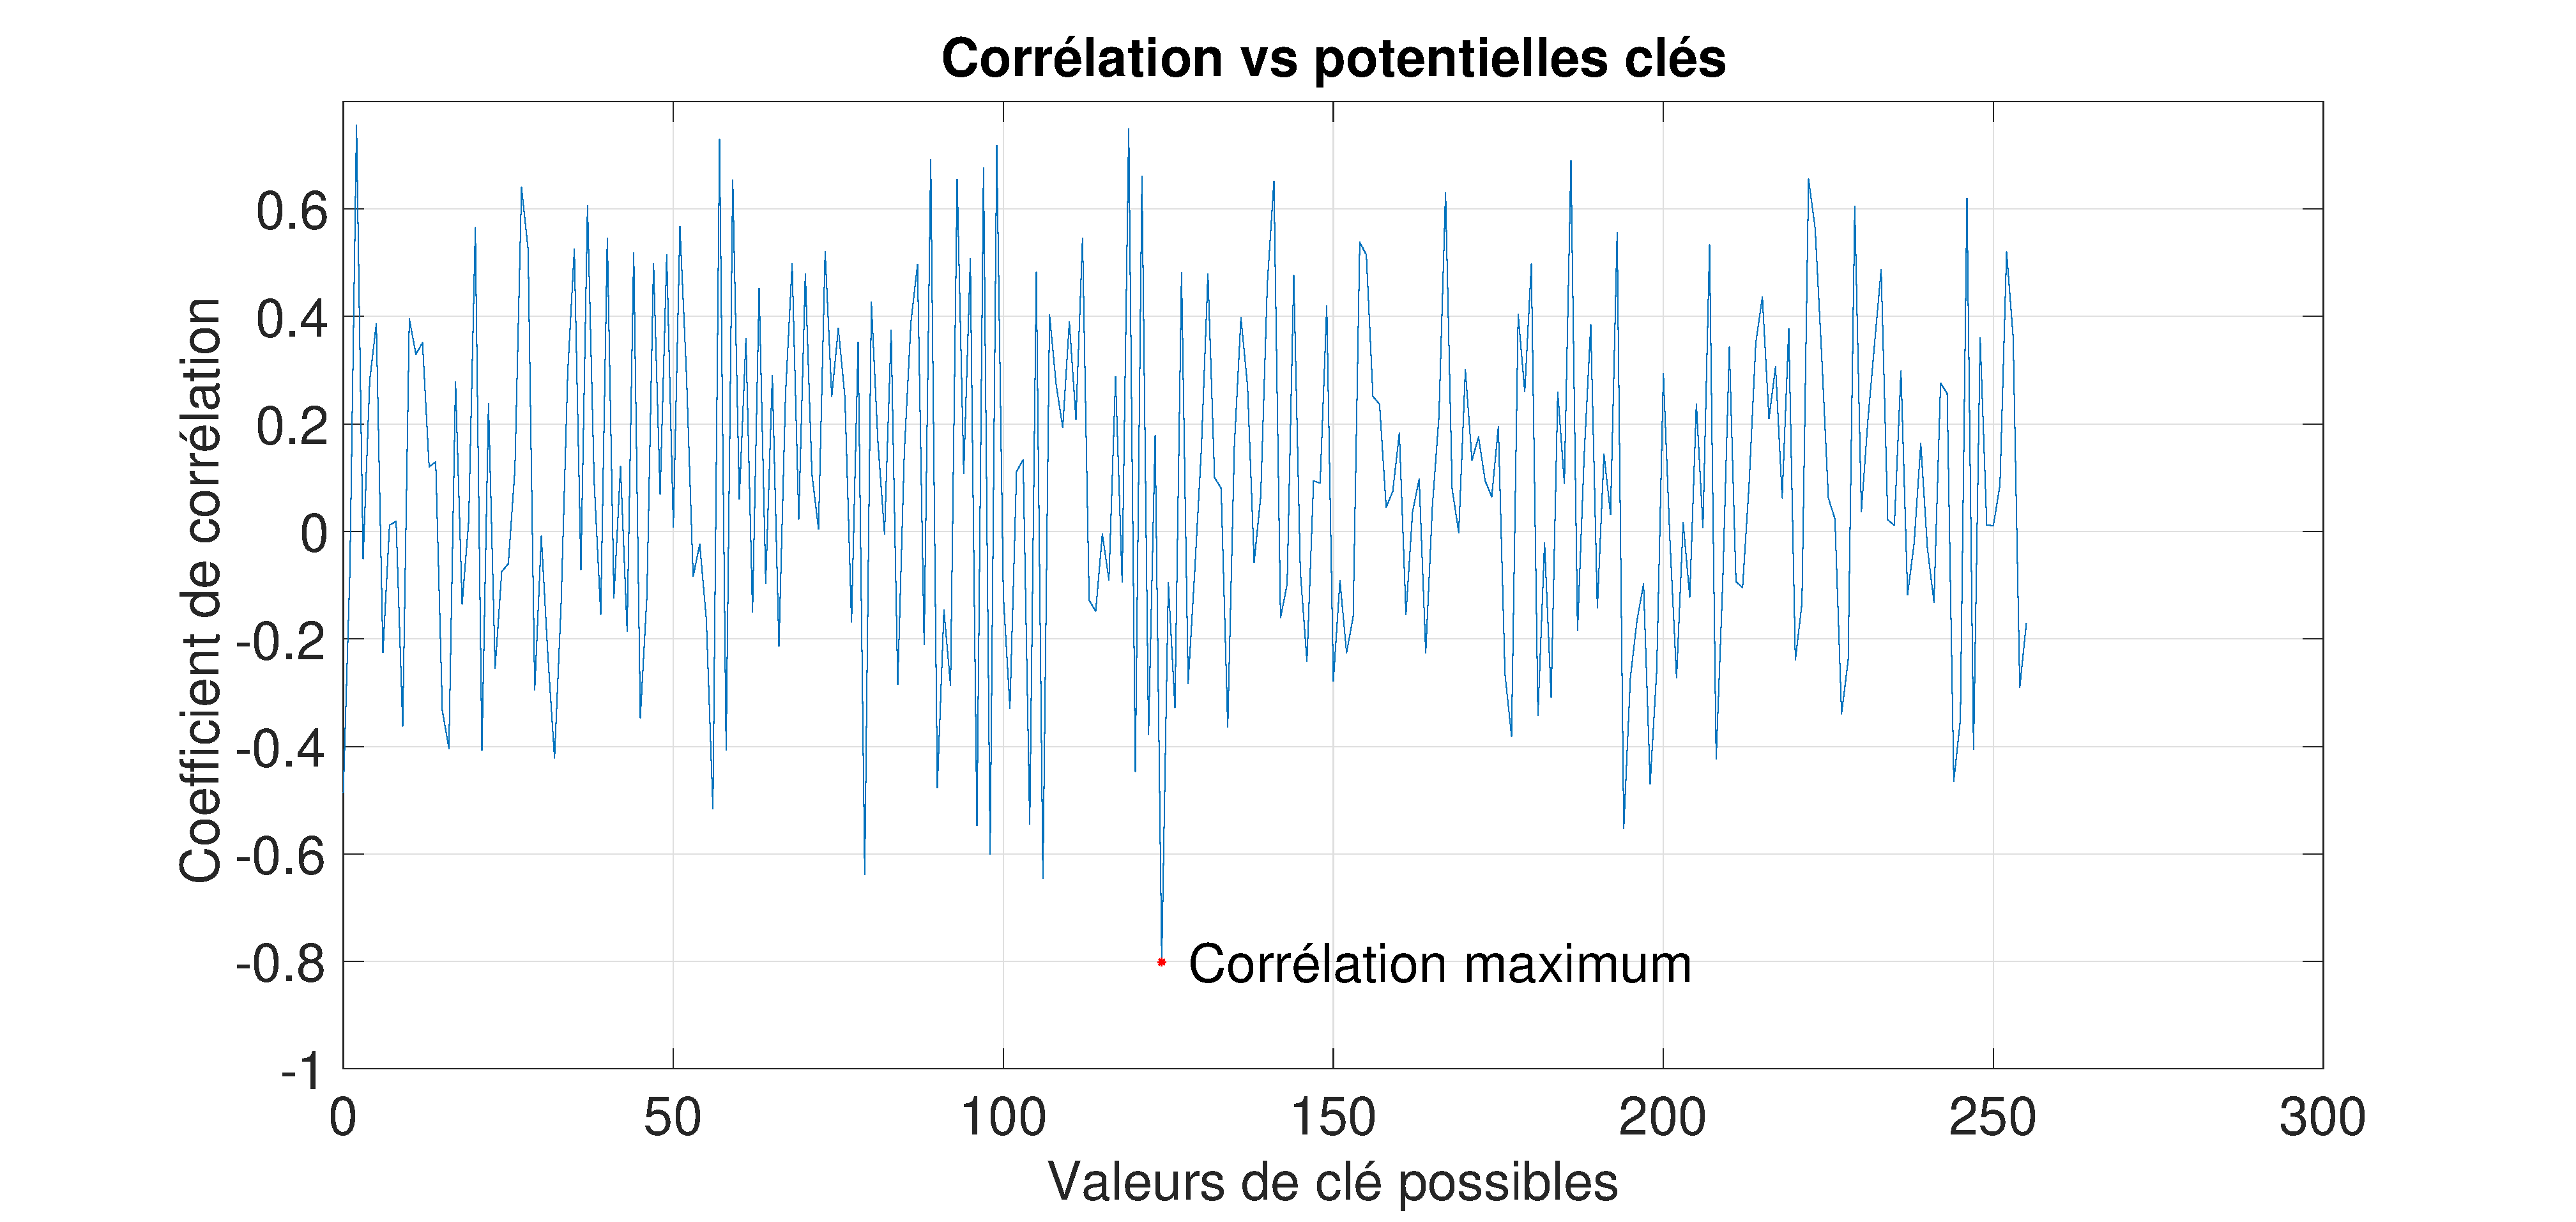
\includegraphics[width=1.05\textwidth]{image/10}    \caption{Coefficient de corrélation en fonction de la valeur de la clé lorsqu'on analyse 10 traces.}    \label{fig:10}
\end{figure}

\begin{figure}[htbp]
    \centering
    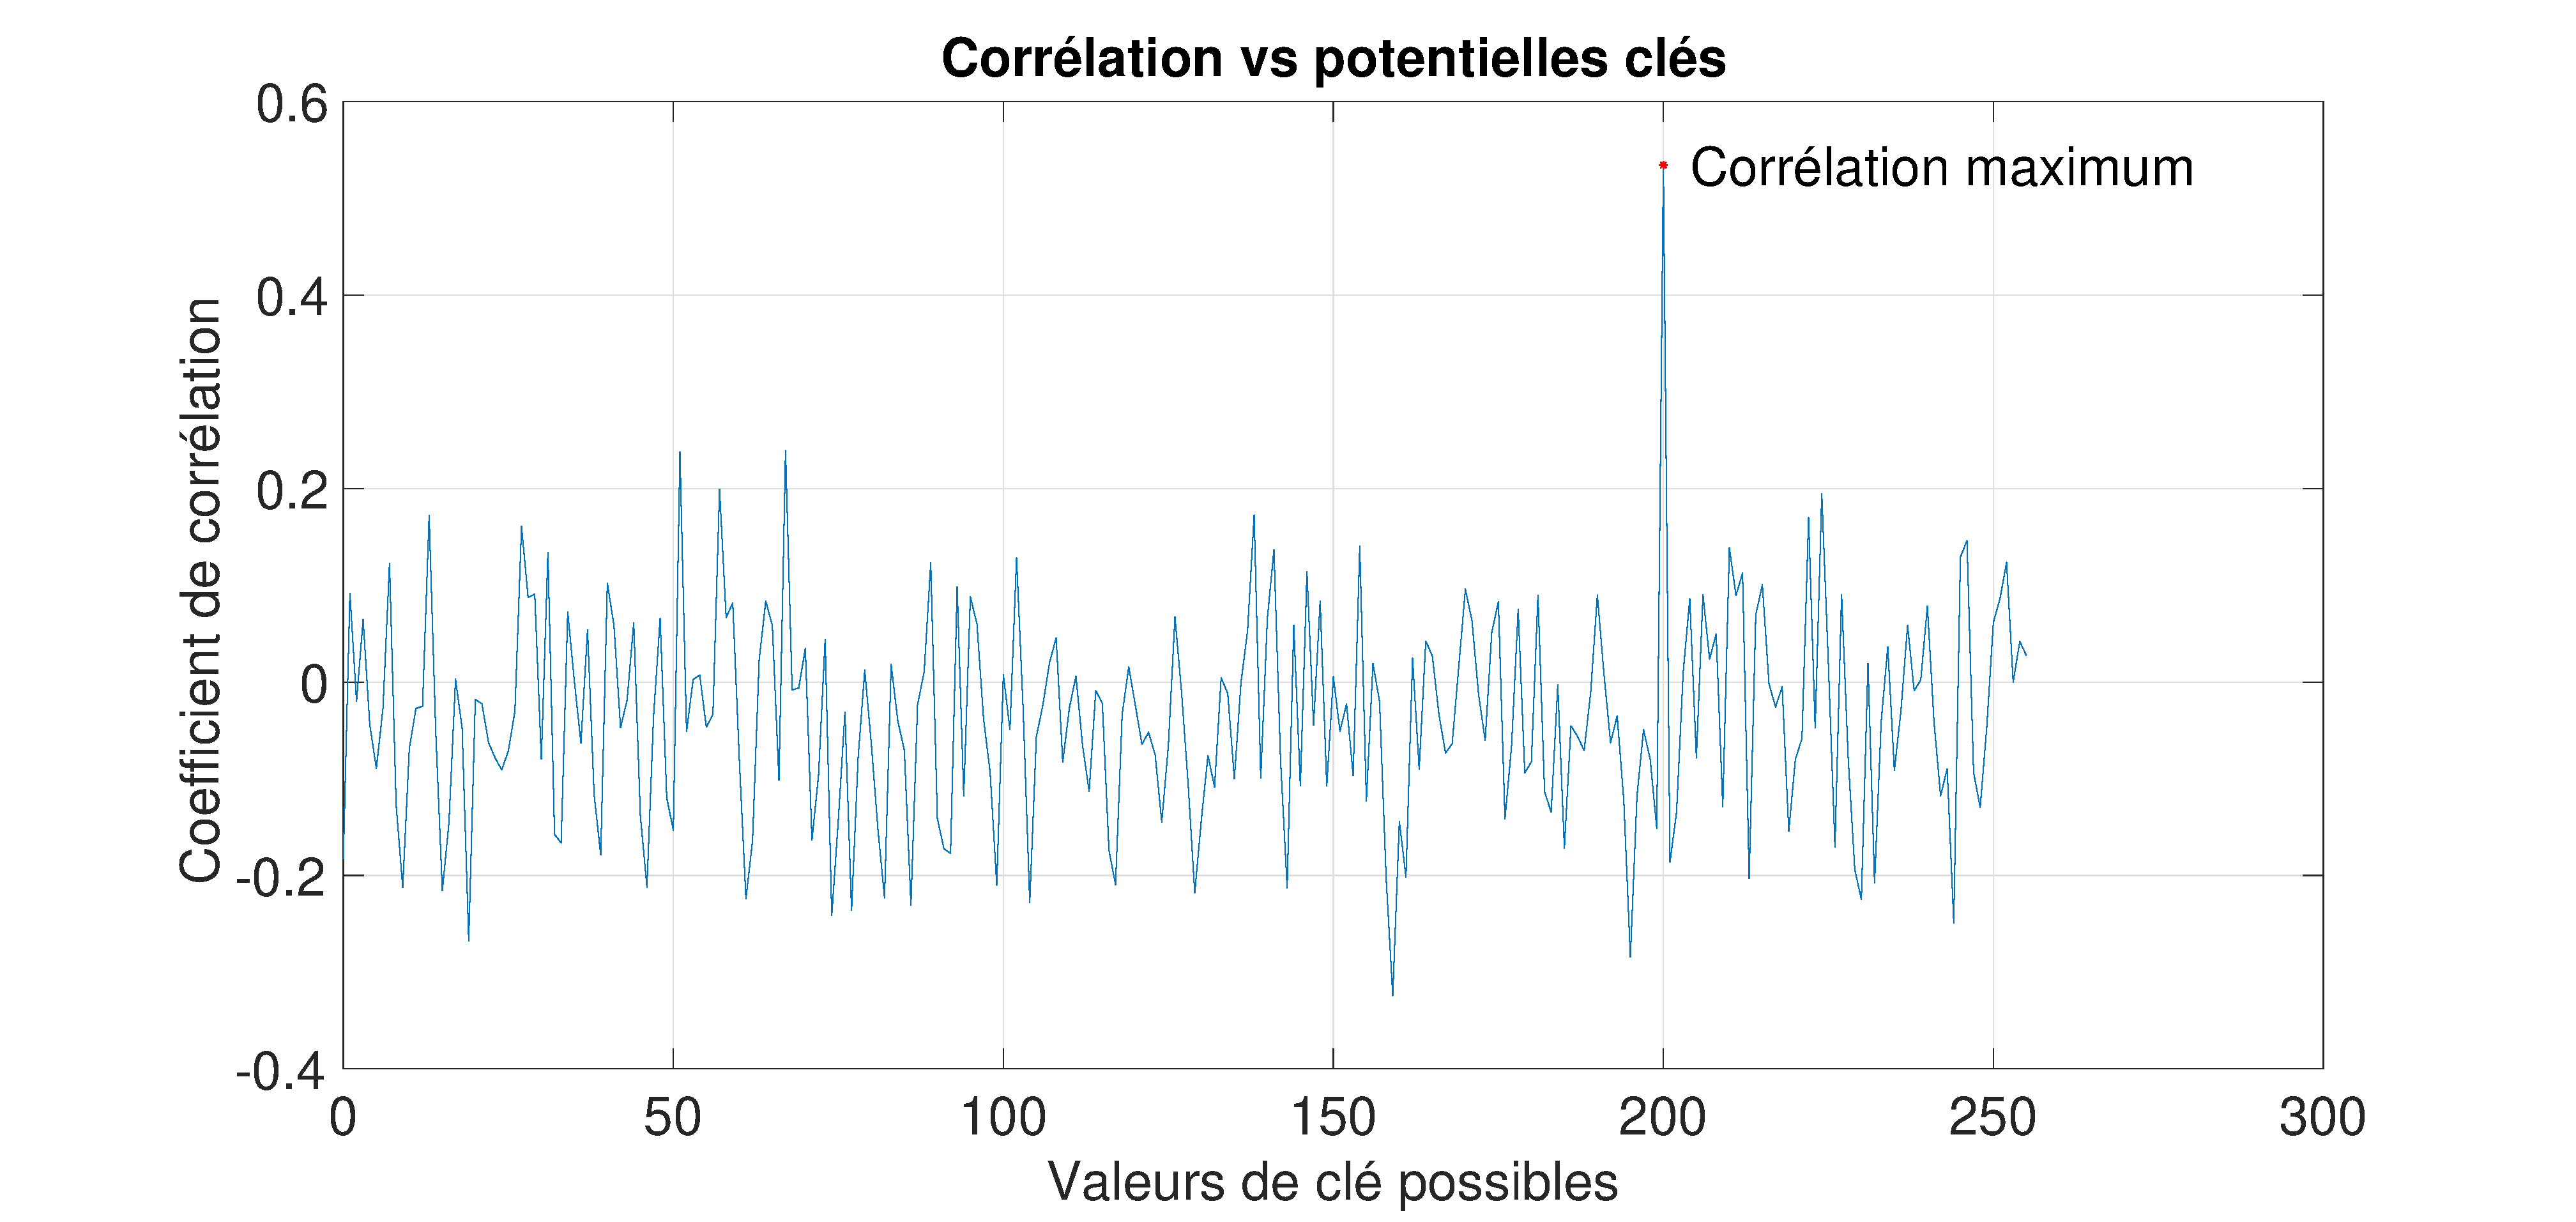
\includegraphics[width=1.05\textwidth]{image/100}    \caption{Coefficient de corrélation en fonction de la valeur de la clé lorsqu'on analyse 100 traces.}    \label{fig:100}
\end{figure}

\begin{figure}[htbp]
    \centering
    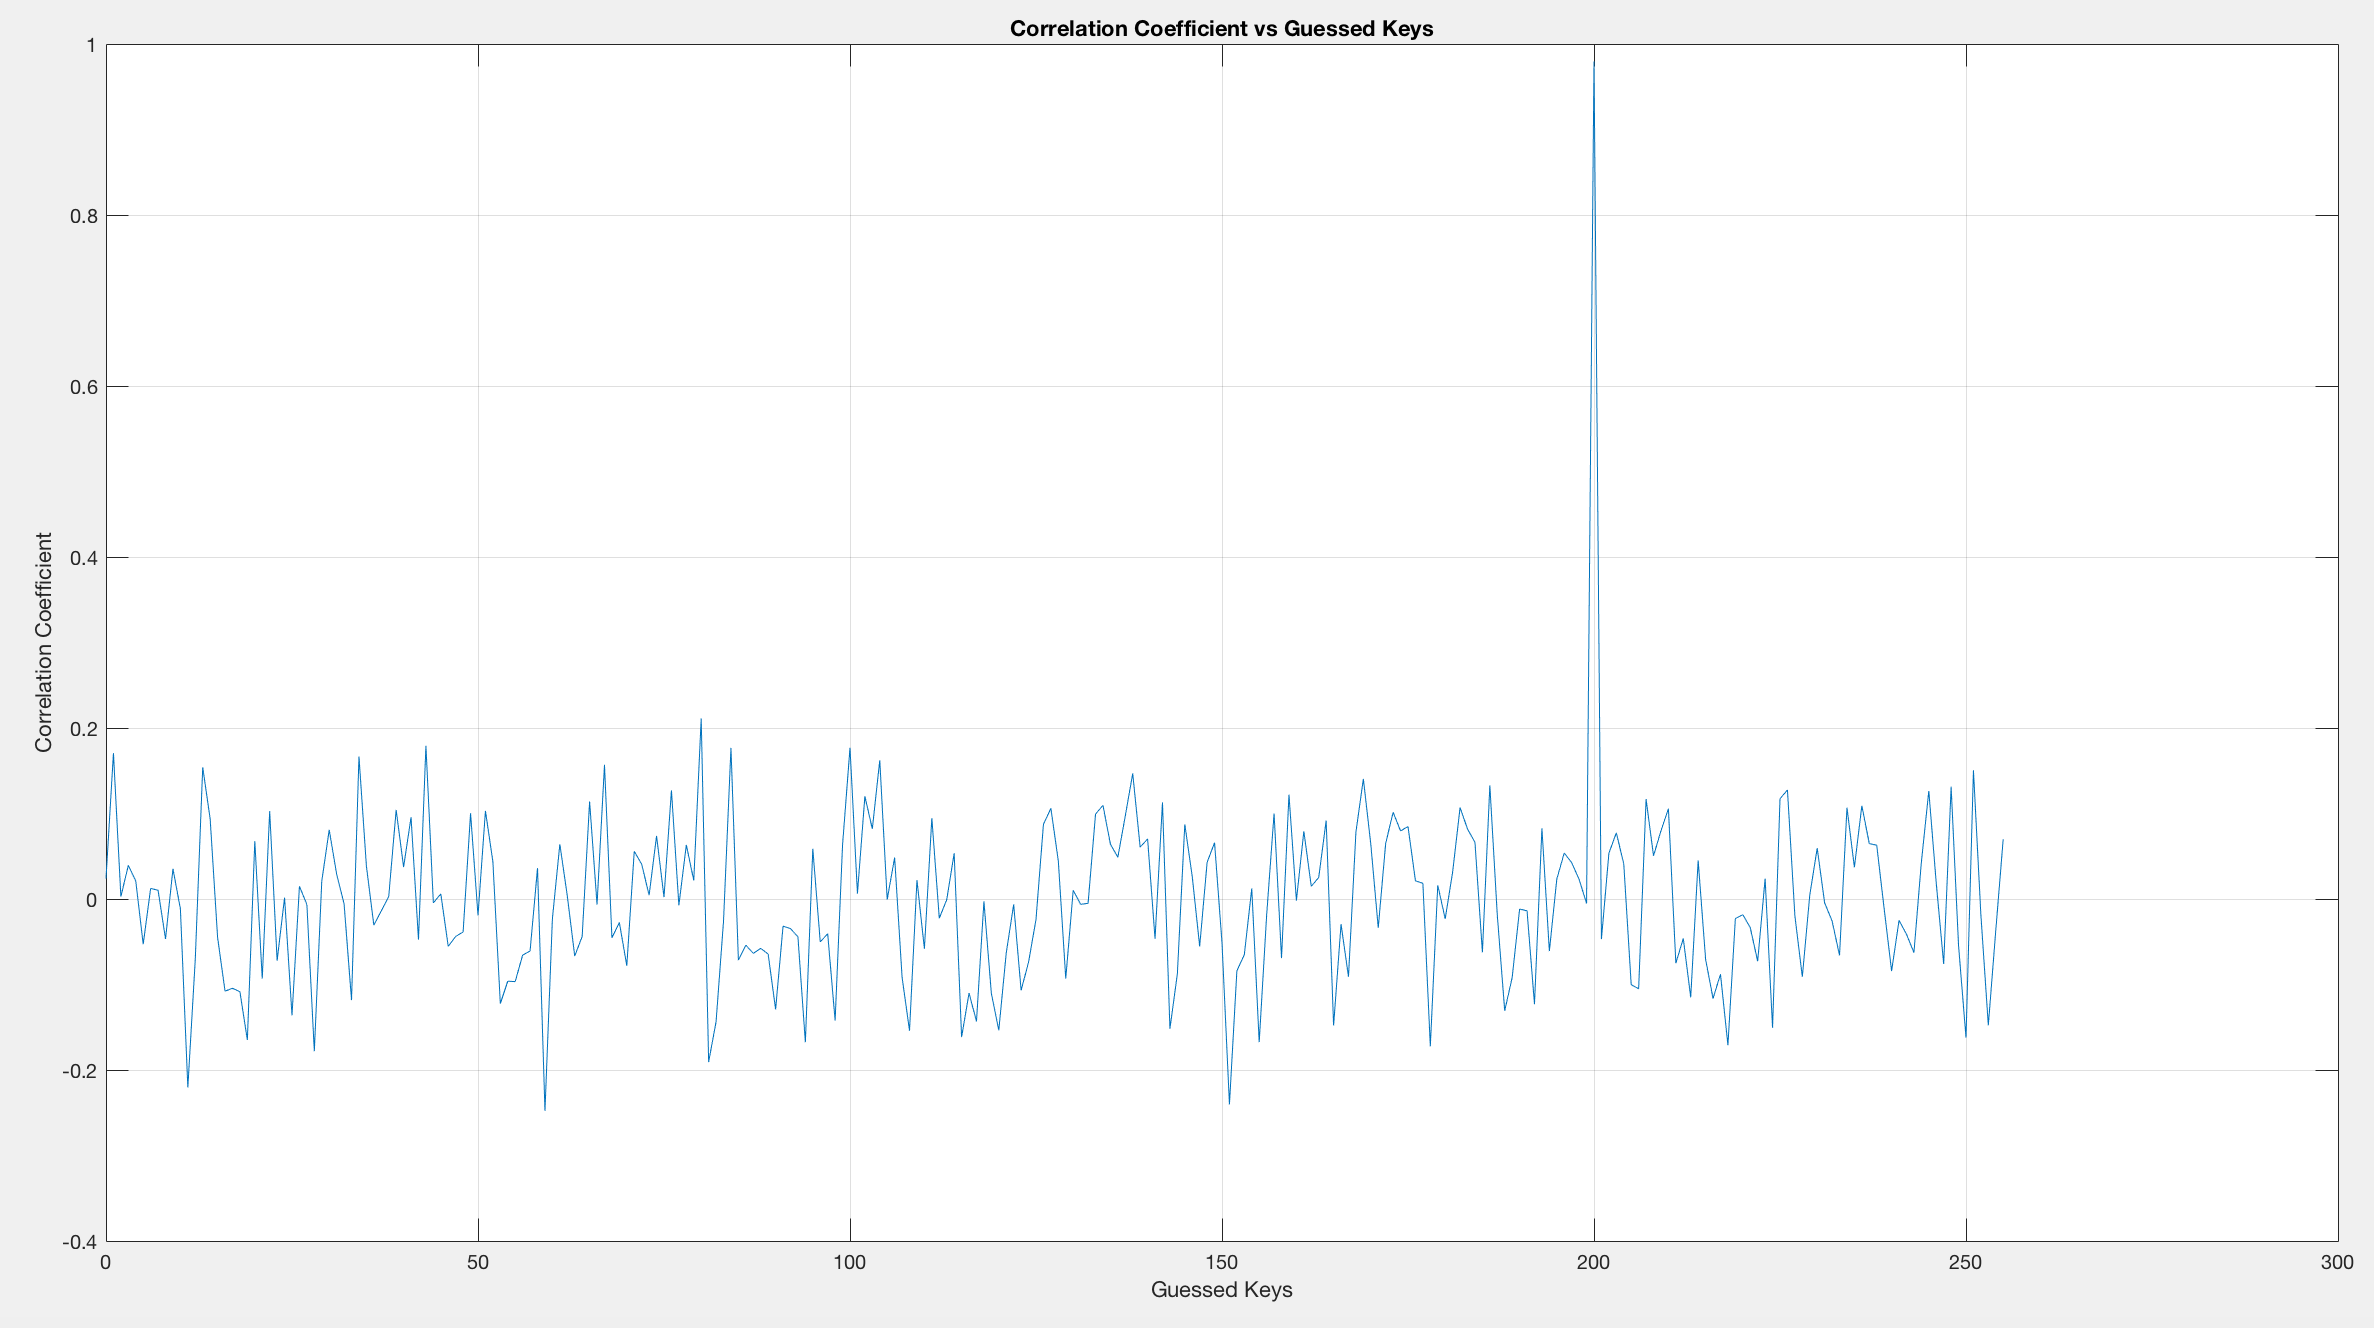
\includegraphics[width=1.05\textwidth]{image/1000}    \caption{Coefficient de corrélation en fonction de la valeur de la clé lorsqu'on analyse 1000 traces.}    \label{fig:1000}
\end{figure}


\newpage

\subsection{Notions de statistiques et de t-test}

Être capable d'analyser les traces de puissance d'un point de vue statistique est une étapes primordiale dans les side-channel attacks.

\subsection{Simulation d'un t-test sur MATLAB}


\newpage
%%%%%%%%%%%%%%%%%%%%%%%% Partie 4 - Conclusion %%%%%%%%%%%%%%%
\section{Conclusion}


\newpage
%%%%%%%%%%%%%%%%%%%%%%%% CREDITS %%%%%%%%%%%%%%%%%%%%
\pagebreak
\phantomsection
\section*{Crédits}
\addcontentsline{toc}{section}{Crédits}

\begin{itemize}
\item Figure~\ref{fig:sigmaDelta} provenant de :\\*
Le blog officiel de Texas Instrument :
\url{https://e2e.ti.com/blogs_/archives/b/precisionhub/archive/2015/01/21/delta-sigma-adc-basics-understanding-the-delta-sigma-modulator}

\item Figure~\ref{fig:classeD} provenant de :\\*
Par Yves-Laurent (Travail personnel) [GFDL (\url{http://www.gnu.org/copyleft/fdl.html}),
CC-BY-SA-3.0 (\url{http://creativecommons.org/licenses/by-sa/3.0/})], de Wikimedia Commons

\item Figure~\ref{fig:filtreLowpass} provenant de :\\*
Par Inductiveload (Travail personnel) [Public domain], de Wikimedia Commons

\item Figure~\ref{fig:filtreHighpass} provenant de :\\*
Par Toriicelli (Travail personnel) [Public domain], de Wikimedia Commons

\item Figure~\ref{fig:IntegPur} provenant de :\\*
Par Daniel Braun [GFDL (\url{http://www.gnu.org/copyleft/fdl.html}),
CC-BY-SA-3.0 (\url{http://creativecommons.org/licenses/by-sa/3.0/}) ou
CC BY 2.5 (\url{https://creativecommons.org/licenses/by/2.5})], de Wikimedia Commons
\end{itemize}

%%%%%%%%%%%%%%%%%%%%%%%% REFERENCES %%%%%%%%%%%%%%%%%%%%
\phantomsection
\section*{Références}
\addcontentsline{toc}{section}{Références}

\begin{itemize}
\item \url{https://www.emse.fr/~dutertre/documents/synth_AES128.pdf}
\item \url{https://www.j3ea.org/articles/j3ea/pdf/2012/01/j3ea12004.pdf}
\item Attaques par canaux auxiliaires : nouvelles attaques, contre-mesures et mises en oeuvre (thèse)
\item From Improved Leakage Detection to the Detection of Points of Interests in Leakage Traces
\item 
\item 
\end{itemize}


\end{document}
